\newpage
\section{Screenshots}

\begin{center}
	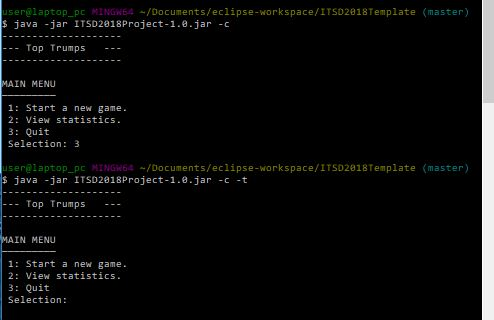
\includegraphics[scale=0.7]{S0010_GameInit}
	\captionof{figure}{Game Initialisation.}
\end{center}
\begin{center}
	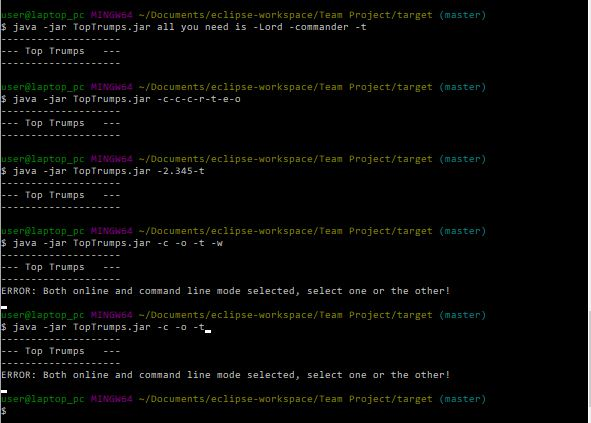
\includegraphics[scale=0.4]{S0010_GameInitAnti}
	\captionof{figure}{Game Initialisation with wrong flag.}
\end{center}
\begin{center}
	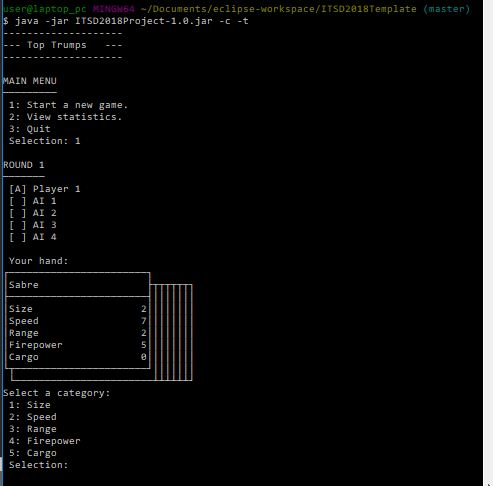
\includegraphics[scale=0.6]{S0010_MainMenu}
	\captionof{figure}{Main Menu with correct integer.}
\end{center}
\begin{center}
	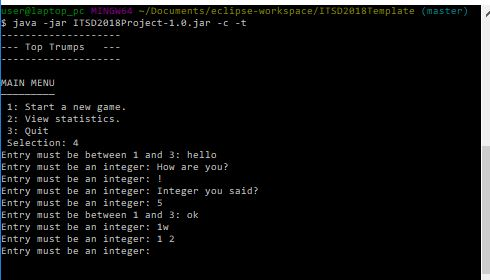
\includegraphics[scale=0.8]{S0010_MainMenuAnti}
	\captionof{figure}{Main Menu with incorrect integer.}
\end{center}
\begin{center}
	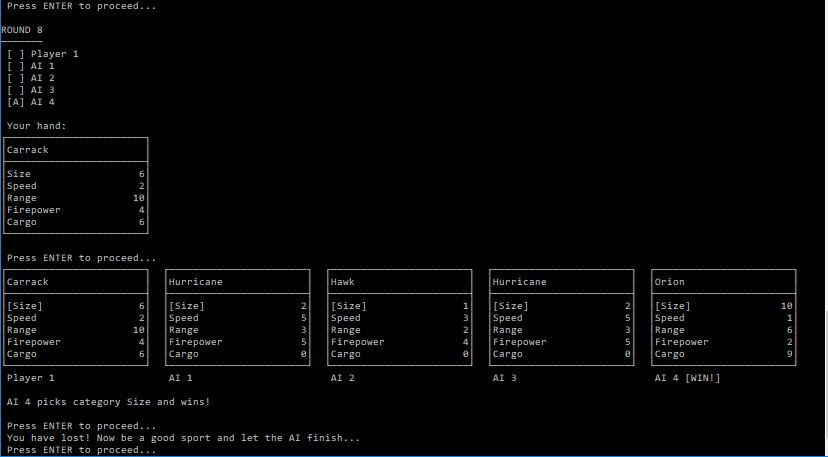
\includegraphics[scale=0.5]{S0030_S0040_RoundInfo}
	\captionof{figure}{Round information and human player is eliminated.}
	\label{figure:cmd_winner}
\end{center}
\begin{center}
	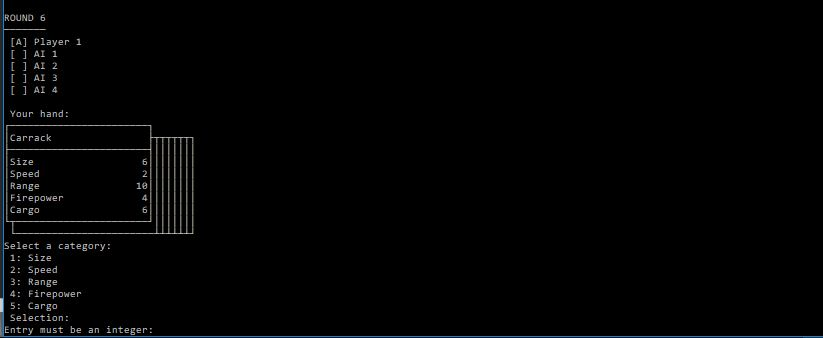
\includegraphics[scale=0.5]{S0030_HumanActive}
	\captionof{figure}{Human player is active player and has to select a category.}
	\label{figure:cmd_play}
\end{center}
\begin{center}
	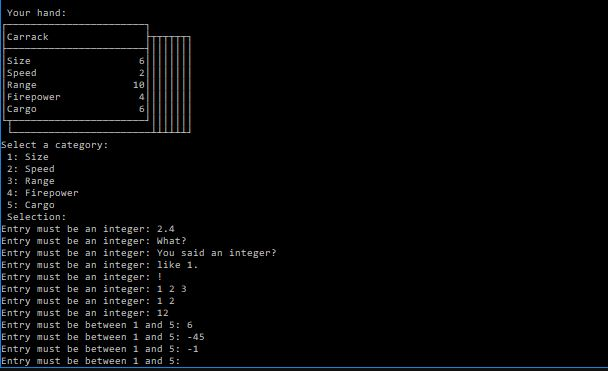
\includegraphics[scale=0.6]{S0030_WrongInput}
	\captionof{figure}{Human player is active player and enters wrong integer number.}
\end{center}
\begin{center}
	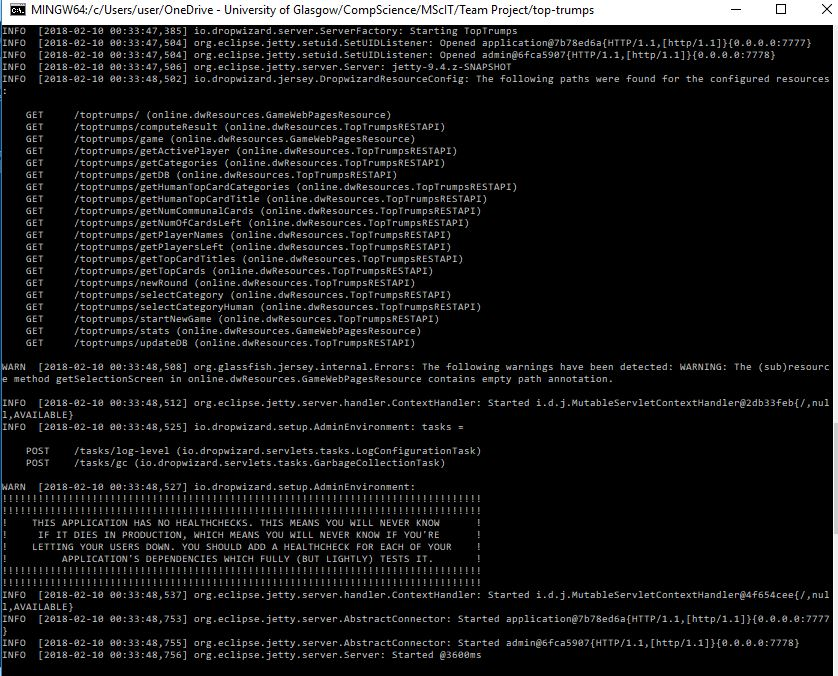
\includegraphics[scale=0.5]{S0200_OnlineMode}
	\captionof{figure}{Initialise online game mode.}
\end{center}
\begin{center}
	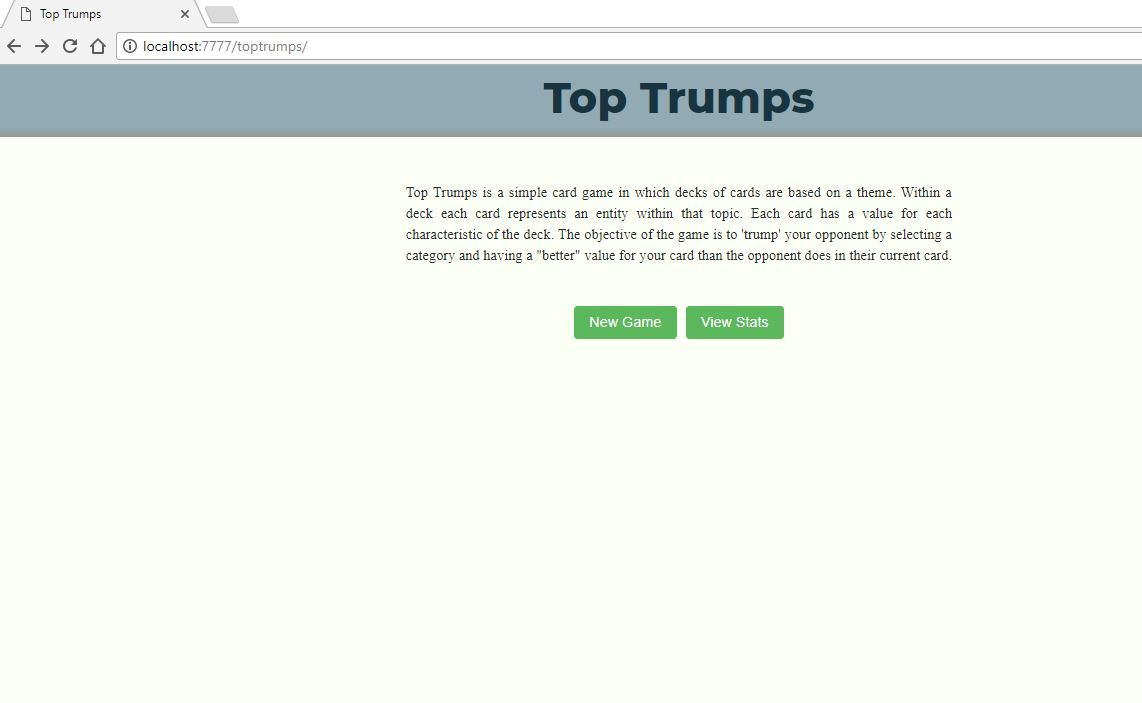
\includegraphics[scale=0.4]{S0200_MainMenu}
	\captionof{figure}{Main menu of the online mode.}
	\label{figure:online_menu}
\end{center}
\begin{center}
	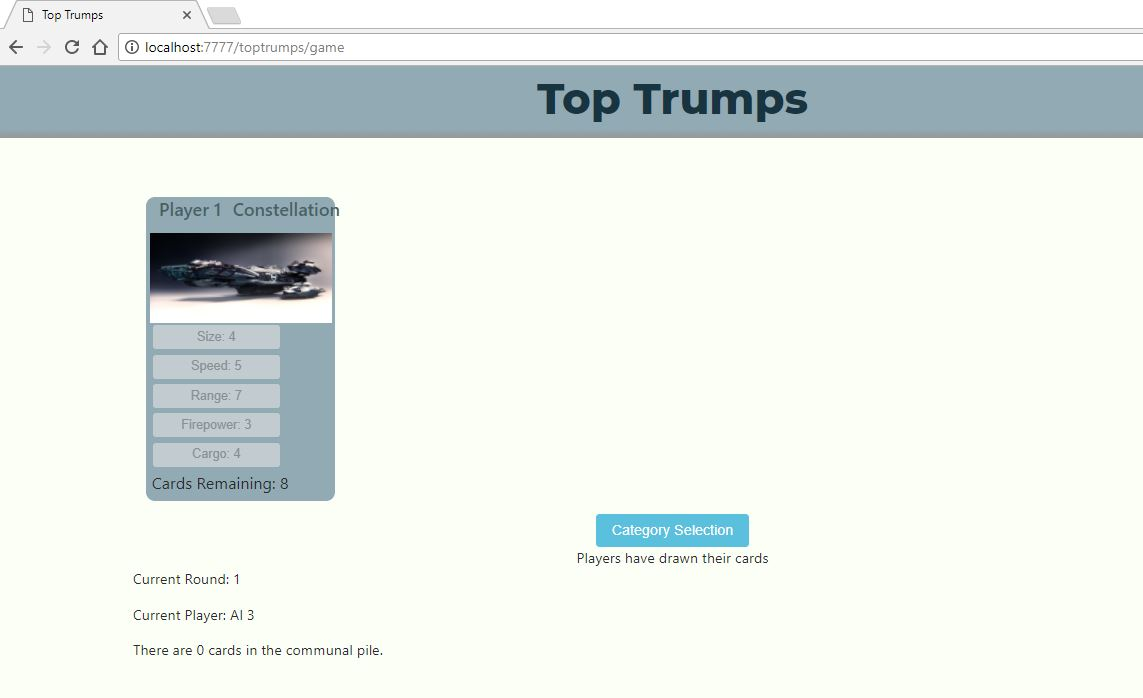
\includegraphics[scale=0.4]{S0220_RoundSet}
	\captionof{figure}{Initialised game, ready to start.}
\end{center}
\begin{center}
	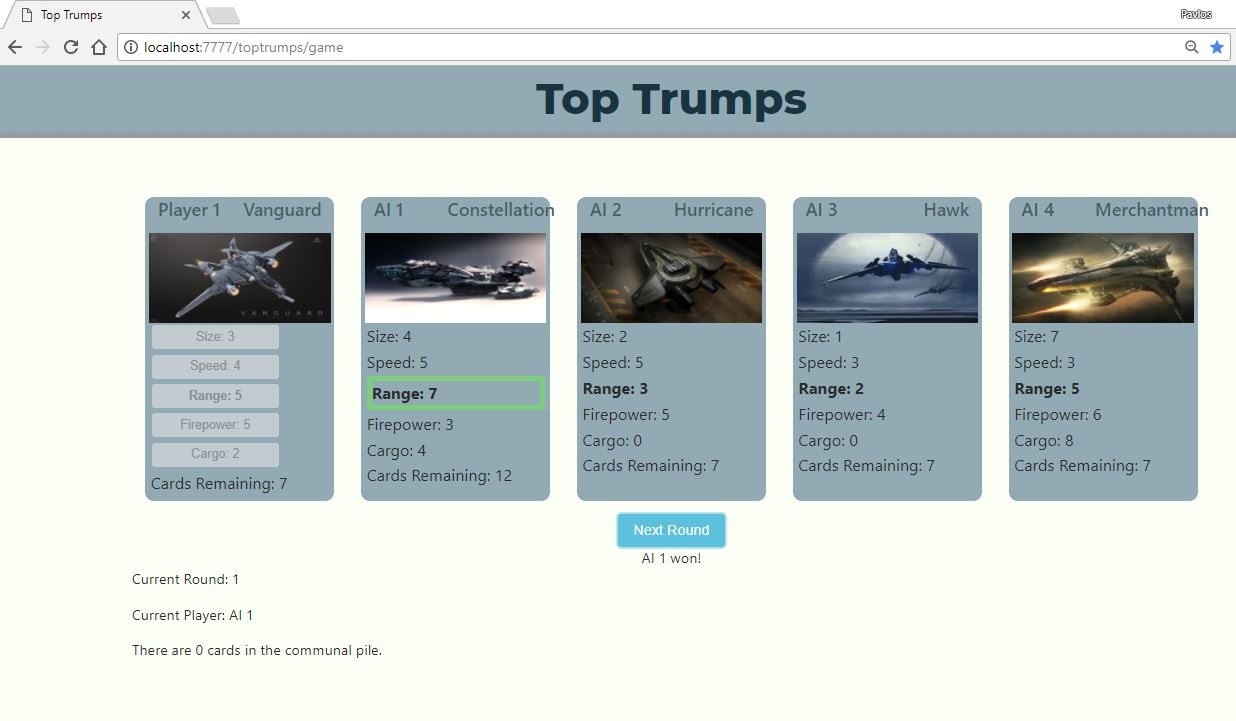
\includegraphics[scale=0.4]{S0220_RoundOutcome}
	\captionof{figure}{Round winner. With bold is the selected category and with the green rectangular indicates the winner}
	\label{figure:online_play}
\end{center}
\begin{center}
	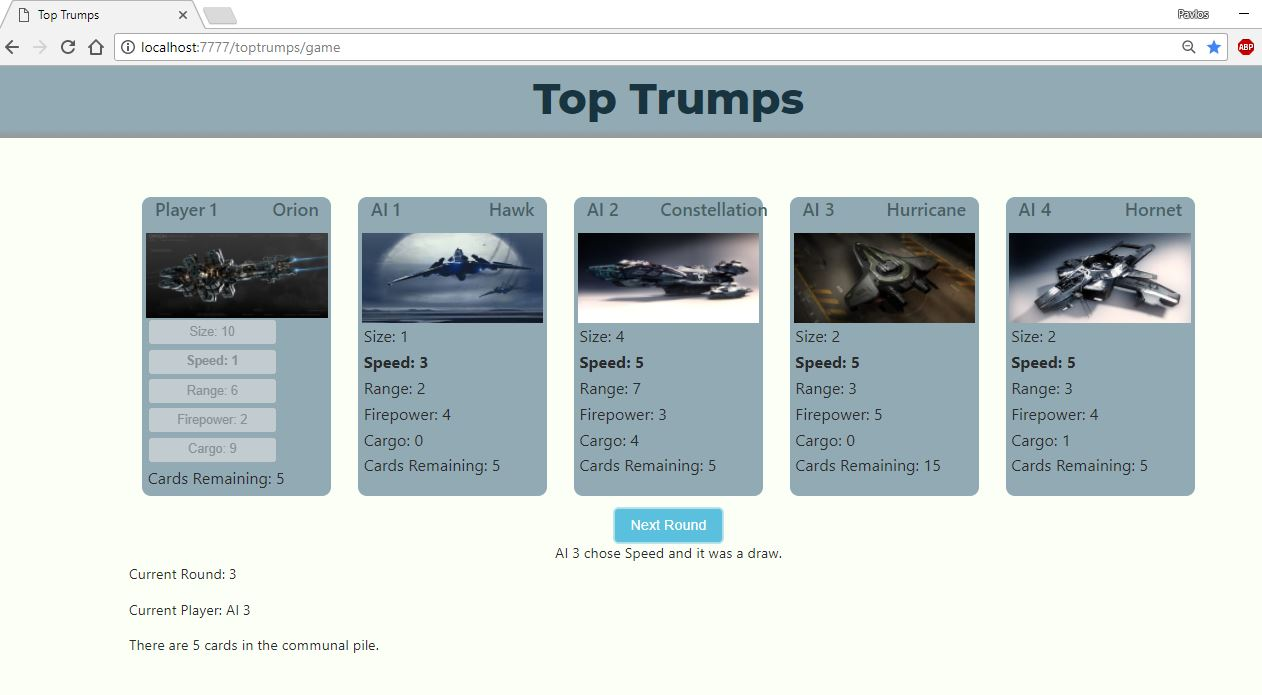
\includegraphics[scale=0.4]{S0240_DrawOnline}
	\captionof{figure}{Draw outcome. With bold is the selected category, there is no green indication of winner and the communal pile stores the cards of the players who are still in the game.}
\end{center}
\begin{center}
	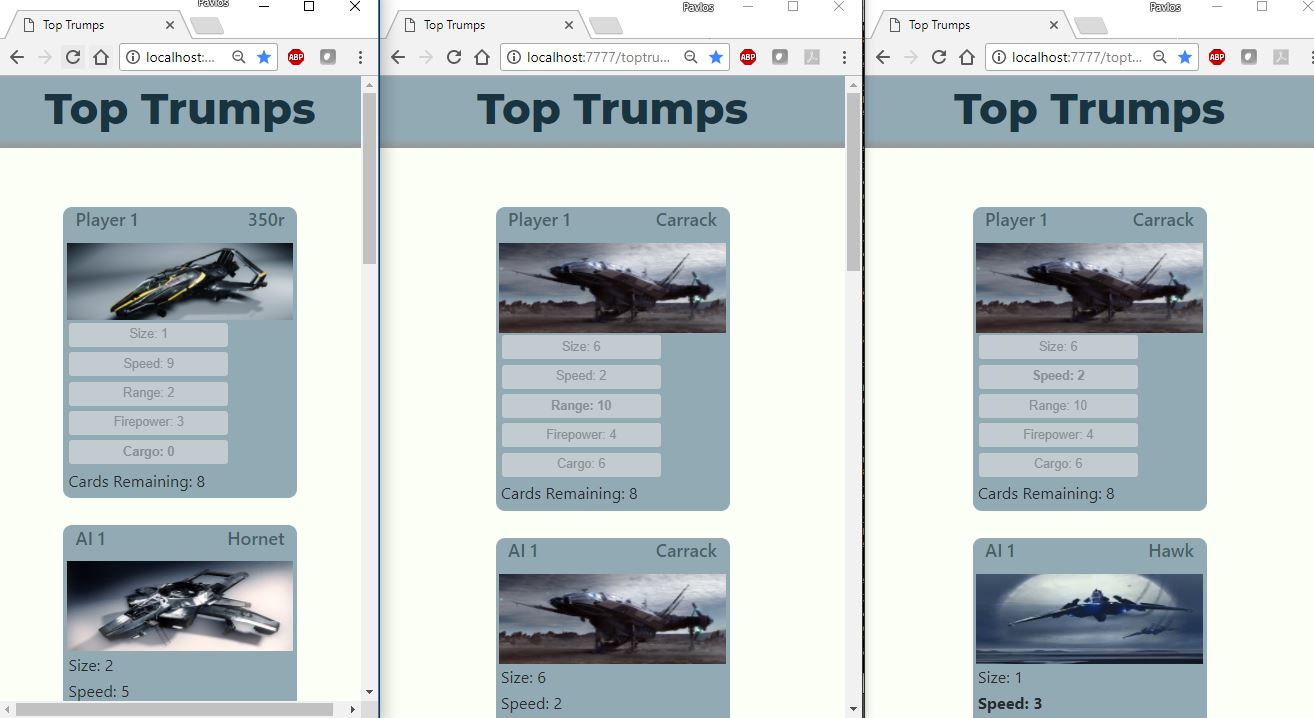
\includegraphics[scale=0.4]{S0250_MultipleGames}
	\captionof{figure}{Multiple games can exist simultaneously in different tabs with game index.}
\end{center}
\begin{center}
	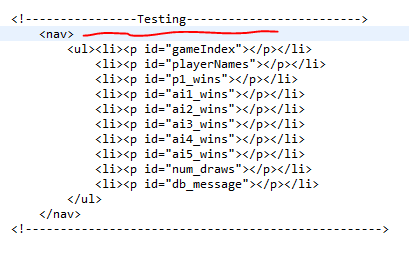
\includegraphics[scale=0.5]{onlineTesting}
	\captionof{figure}{The above variables were not hidden during the development of the, in order to test the functionality of the online mode.}
\end{center}
\begin{center}
	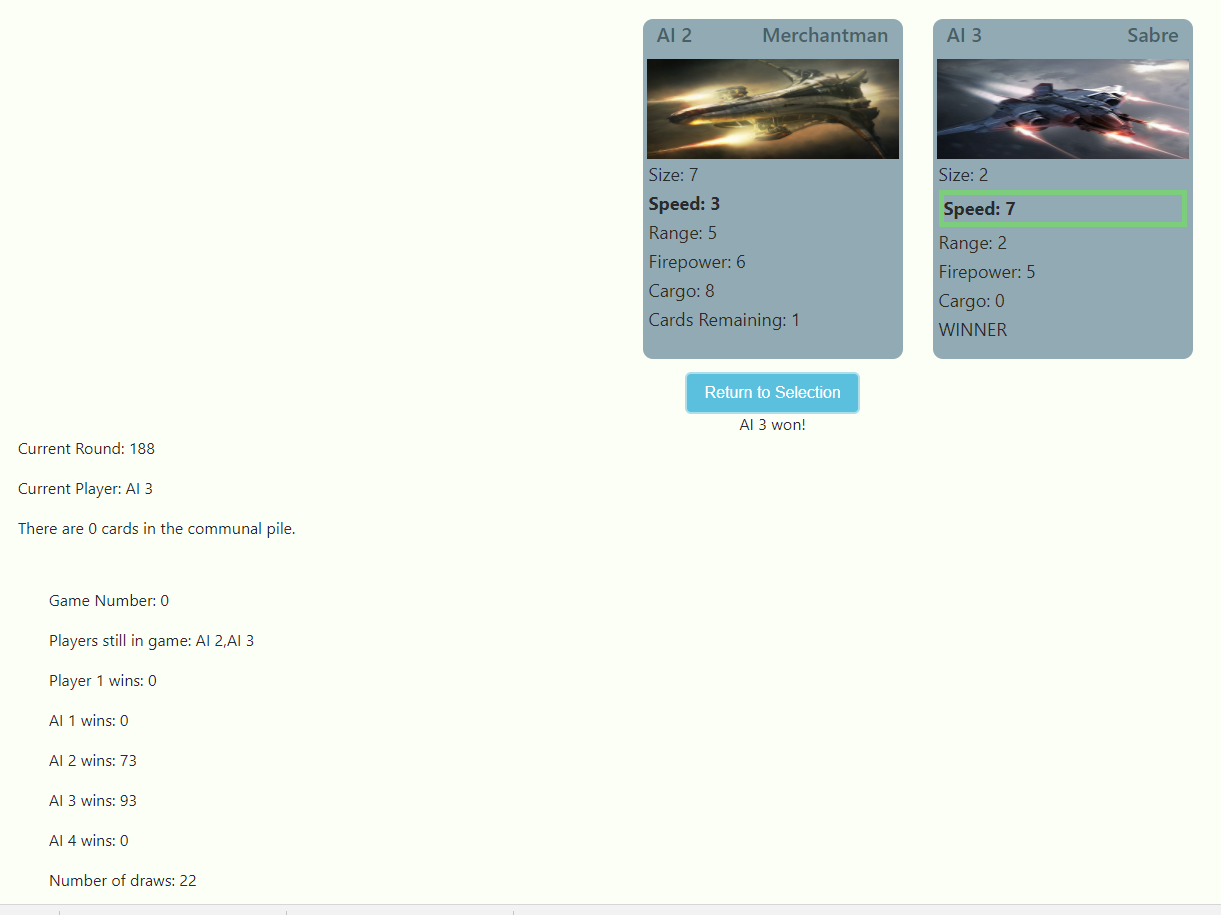
\includegraphics[scale=0.3]{onlineTesting_2}
	\captionof{figure}{This figure is connected with the figure above and provides a clear understanding about the testing.}
\end{center}
Add a cmd line statistics screenshot
\begin{center}
    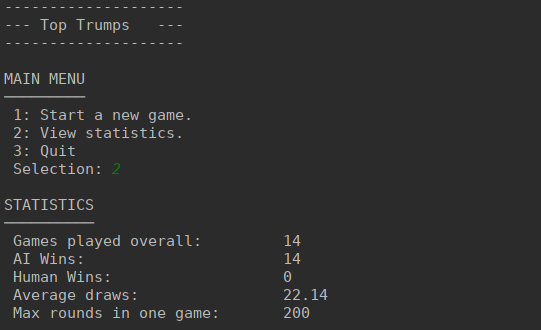
\includegraphics[scale=0.7]{cmd_stats}
    \captionof{figure}{Command Line Statistics View}
    \label{figure:cmd_stats}
\end{center}
\begin{center}
    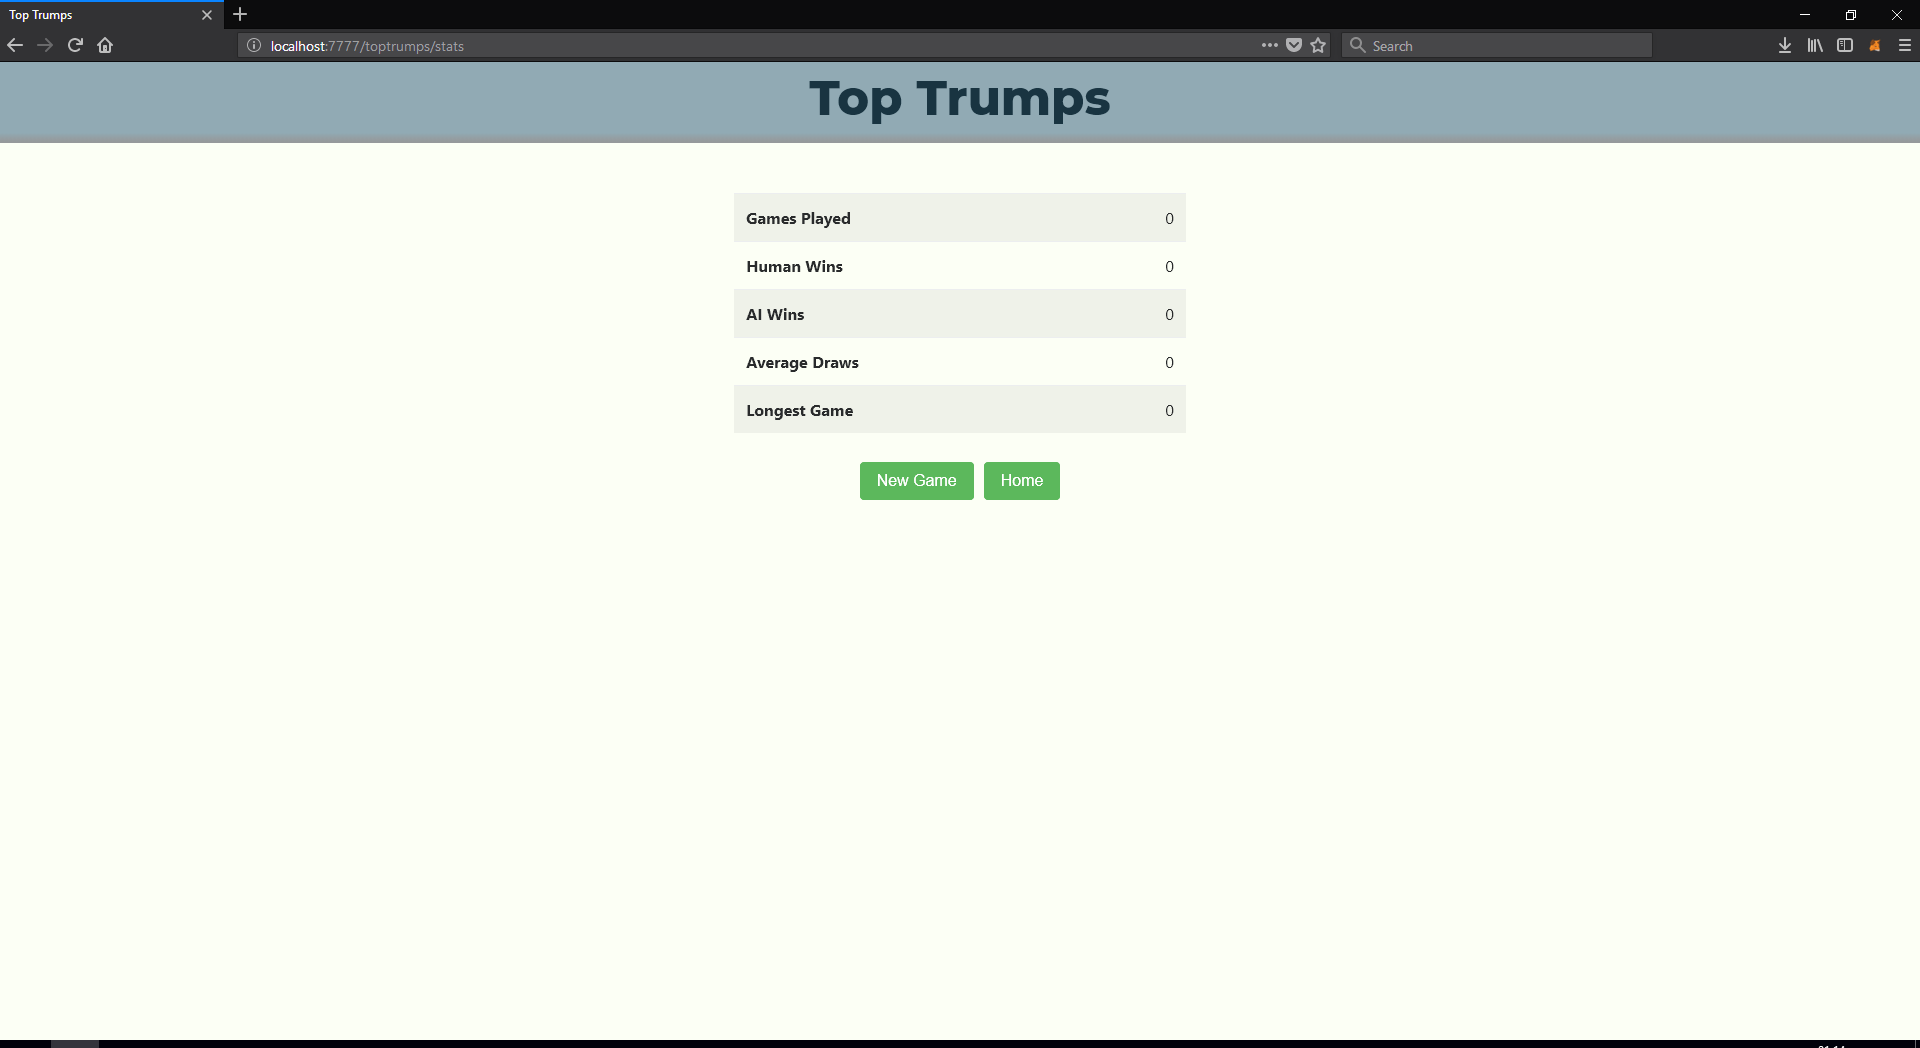
\includegraphics[width=\textwidth]{online_stats}
    \captionof{figure}{Online Statistics View}
    \label{figure:online_stats}
\end{center}


